\documentclass{article}

% if you need to pass options to natbib, use, e.g.:
% \PassOptionsToPackage{numbers, compress}{natbib}
% before loading nips_2016
%
% to avoid loading the natbib package, add option nonatbib:
% \usepackage[nonatbib]{nips_2016}

%\usepackage{nips_2016}

% to compile a camera-ready version, add the [final] option, e.g.:
 \usepackage[final]{nips_2016}

\usepackage[utf8]{inputenc} % allow utf-8 input
\usepackage[T1]{fontenc}    % use 8-bit T1 fonts
\usepackage{hyperref}       % hyperlinks
\usepackage{url}            % simple URL typesetting
\usepackage{booktabs}       % professional-quality tables
\usepackage{amsfonts}       % blackboard math symbols
\usepackage{nicefrac}       % compact symbols for 1/2, etc.
\usepackage{microtype}      % microtypography
\usepackage{graphicx}

\title{Hubble's Tuning Fork: \\A Deep Learning Approach}

% The \author macro works with any number of authors. There are two
% commands used to separate the names and addresses of multiple
% authors: \And and \AND.
%
% Using \And between authors leaves it to LaTeX to determine where to
% break the lines. Using \AND forces a line break at that point. So,
% if LaTeX puts 3 of 4 authors names on the first line, and the last
% on the second line, try using \AND instead of \And before the third
% author name.

\author{
  Brandon Bergerud \\
  Department of Physics and Astronomy\\
  University of Iowa\\
  Iowa City, IA  52242 \\
  \texttt{brandon-bergerud@uiowa.edu} \\
  %% examples of more authors
  \And
  Ossian Mogensen \\
  Department of Computer Science \\
  University of Iowa \\
  Iowa City, IA  52242 \\
  \texttt{ossian-mogensen@uiowa.edu} \\
  %% \AND
  %% Coauthor \\
  %% Affiliation \\
  %% Address \\
  %% \texttt{email} \\
  %% \And
  %% Coauthor \\
  %% Affiliation \\
  %% Address \\
  %% \texttt{email} \\
  %% \And
  %% Coauthor \\
  %% Affiliation \\
  %% Address \\
  %% \texttt{email} \\
}

\begin{document}
% \nipsfinalcopy is no longer used

\maketitle

\begin{abstract}
With the introduction of powerful telescopes such as the Hubble Space Telescope, vast quantities of high-fidelity imagery of remote galaxies have become available. Manual analysis of these images by experts has become infeasible, spawning citizen science projects such as Galaxy Zoo. However, the next generation of telescopes are expected to generate enormous volumes of data, going far beyond the capacity even of crowdsourced volunteers. In this study, we extend the work done on automatic galaxy image classification in the Galaxy Zoo 2 Kaggle challenge by training a convolutional neural network based on the Google Inception architecture, utilizing transfer learning from the popular ImageNet dataset. After re-training the final layers and fine-tuning the weights, the model was evaluated on the Galaxy Zoo 1 and 2 datasets, as well as an expert-annotated dataset, using images from the Sloan Digital Sky Survey. \ldots
\end{abstract}

\section{Introduction}
The size and scope of astronomy datasets has increased dramatically in recent years. The introduction of telescopes such as the Hubble Space Telescope (HST) and projects like the Sloan Digital Sky Survey (SDSS) have given astronomers access to imagery of millions of celestial objects. Traditional methods of data analysis, manually inspecting and classifying celestial objects, have become untenable in the face of this embarrassment of riches of data. 

Astronomers have successfully turned to citizen science projects such as Galaxy Zoo to leverage vast numbers of volunteers to help classify objects. The human visual system can, with little effort or training, provide image recognition capabilities that match or exceed the state of the art in computer image recognition. 

With the dawn of a new generation of telescopes, astronomy is threatened to be deluged in a sea of data. The GAIA spacecraft will produce a 3D map of over 1 billion astronomical objects \citep{2016A&A...595A...1G}. The Thirty Meter Telescope (TMT) \citep{2015RAA....15.1945S} and the 40-meter European Extremely Large Telecope (E-ELT) will view the visible universe at unprecedented depth. The Large Synoptic Survey Telescope (LSST) is estimated to generate 15 TB of data each night as it surveys the entire night sky \citep{2009AAS...21346003I}. Even these vast sums of data pale in comparision to the monsuvian output expected from the Square Kilometer Array (SKA). Such enormous sums of data are beyond the ability of crowdsourcing to handle: they can only be handled by leveraging supercomputers, sophisticated algorithms, and machine learning.

The Galaxy Zoo Kaggle challenge was a competition in 2013 to produce a machine learning model that could replicate the classifications of citizen science volunteers on a dataset of 70,000 galaxy images captured by SDSS. The top models performed very well in this challenge, but several questions remain. Can the galaxy classification scheme used by Galaxy Zoo 2 (GZ2) (Figure \ref{fig:GZ2tree}) be effectively mapped to astronomical classification schemes such as Hubble's Tuning Fork, or the more complex de Vaucouleurs system? Will machine learning models trained on the Galaxy Zoo dataset generalize well to other sources? 


\begin{figure}[h]
  \centering
	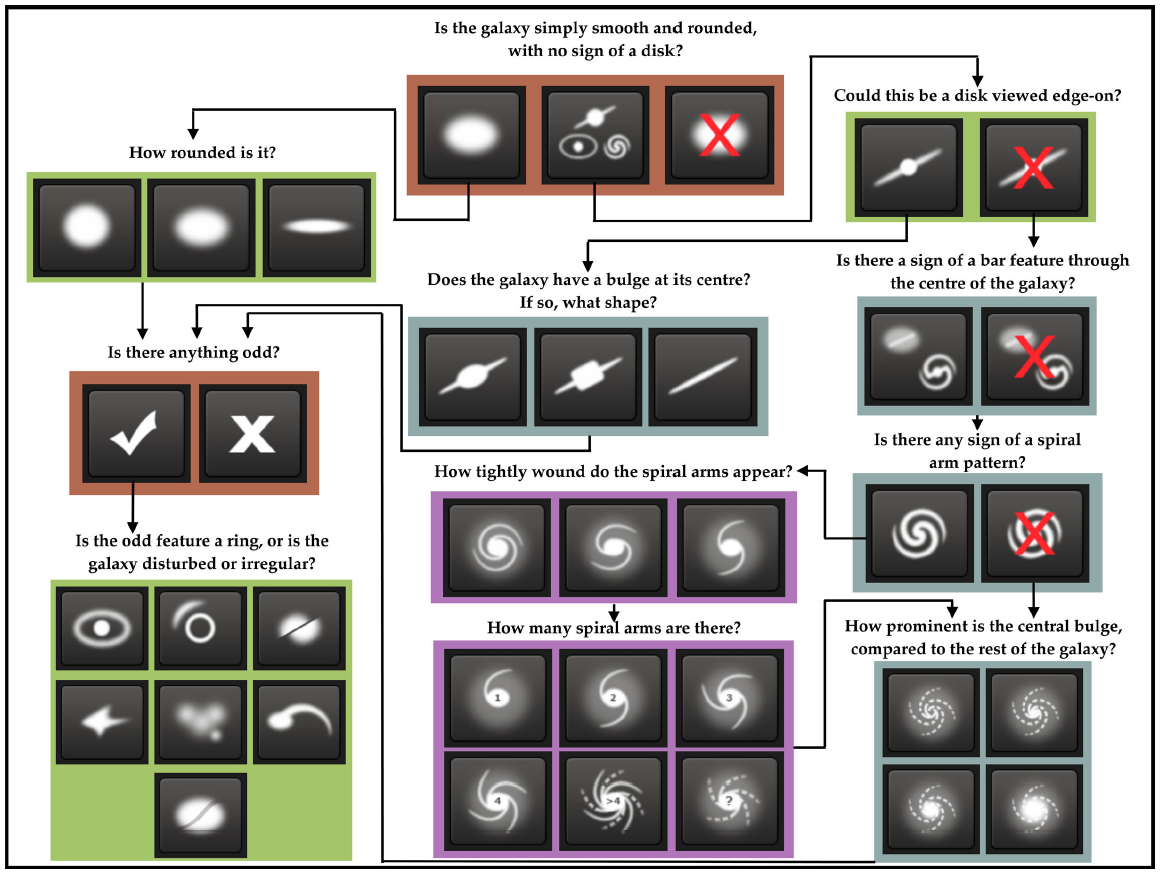
\includegraphics[width=100mm]{../img/GZ2_tree.png}
  \caption{The Galaxy Zoo 2 decision tree. Image from \cite{2013MNRAS.435.2835W}.}
  \label{fig:GZ2tree}
\end{figure}

To answer these questions, we will use the results from the Galaxy Zoo “decision tree” classification scheme to map galaxies onto the Hubble Tuning Fork (Figure \ref{fig:tuningFork}). A machine learning system based on the Google’s Inception architecture for convolutional neural networks was trained on the Galaxy Zoo dataset to produce Tuning Fork classifications and tested against a 3rd party dataset of images classified manually by experts.

\begin{figure}[h]
  \centering
	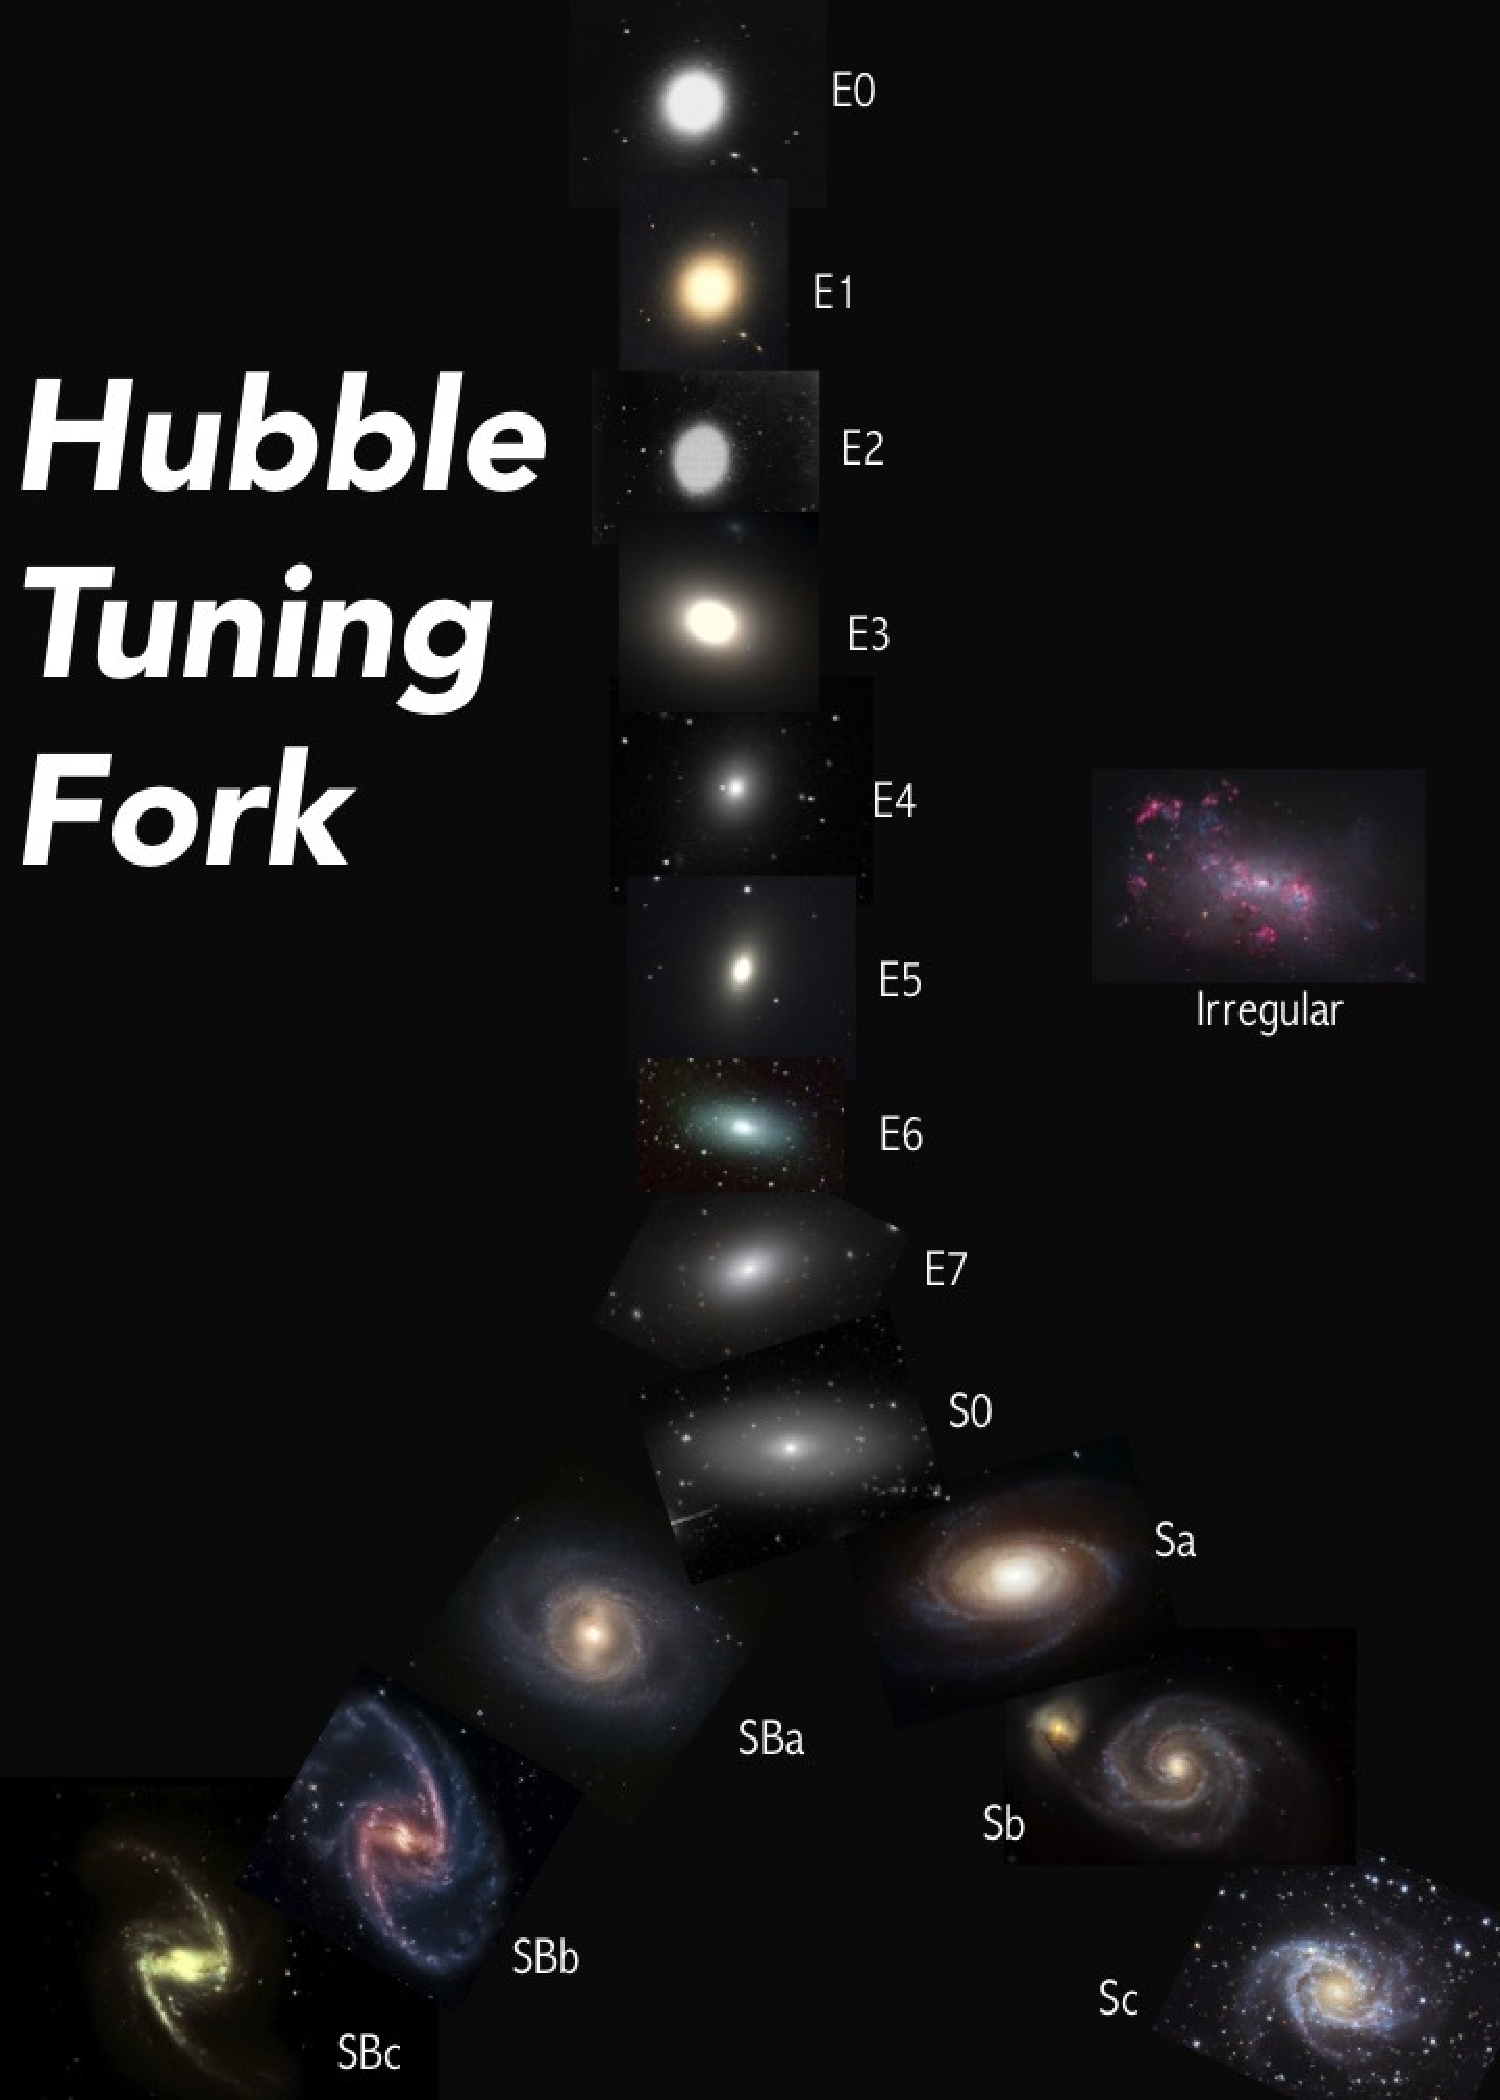
\includegraphics[width=100mm]{../img/tuningFork.pdf}
  \caption{Hubble's tuning fork model. From http://ay17-chusic.blogspot.com/2015/10/20-hubble-tuning-fork.html}
  \label{fig:tuningFork}
\end{figure}


\section{Related Work}
\label{gen_inst}
In the astronomical community, the few automated galaxy classification systems have relied on more tradition methods, focusing on aggressive feature extraction algorithms making use of domain knowledge to identify relationships among galaxies. These, however, have tended to focus on the more narrow classification of spirals and ellipticals, occasionally including edge-on spirals and irregular galaxies, and often work with much smaller datasets (see \citealt{2015MNRAS.450.1441D} for a discussion). \cite{2016ApJS..223...20K} were rather unique when they made use of the "super clean" galaxies from the Galaxy Zoo 1 catalog \citep{2008MNRAS.389.1179L} to classify 3 000 000 galaxies into spirals and ellipticals.

While the top methods achieve $\sim95\%$ accuracy when separating ellipticals and spirals, they tend to perform much worse when the number of categories increases \citep{2004MNRAS.349...87D}.

%One example of the simple classification approach was done by \cite{2016ApJS..223...20K}, who, rather uniquely, made use of the ``super clean" galaxies from the Galaxy Zoo 1 catalog \citep{2008MNRAS.389.1179L} to classify 3 000 000 galaxies into spirals and ellipticals.

\cite{stanford}, students in Prof. Ng's machine learning class at Stanford, recently looked at several machine learning methods for classifying galaxies using the GZ2 dataset. While acknowledging the difficulty of directly classifying to the Hubble types, they sought to bridge the gap by modeling certain features, such as "roundness" and "diskiness". They utilized the GZ2 decision tree to assign each galaxy to one of five categories: disc, spiral, elliptical, round, and other. In their preprocessing stage, images were cropped to reduce the file size, as well as reduce the number of nearby sources contaiminating the images. The galaxies were then rotated to align the principle axis, before proceeding with a background subtraction.

To further reduce the dimensionality of the problem, the authors applied principal component analysis (PCA), selecting the top 125 components to maintain $>99\%$ of the variance. To classify the galaxies, they utilized a support vector machine (SVM) with a radial basis function (RBF) kernel, a decision tree, random forest, k-nearest neighbors, and an AdaBoost classifier, determining the classification accuracy using 10-fold cross validation. Overall, random forest produce the best results, achieving 67\% accuracy. The poor success rate lead them to look into predicting probabilities (regression) rather than directly modeling the classes, similar to the Galaxy Zoo Kaggle challenge. They achieved better results in this regard, attaining $\sim 95\%$ accuracy.

Overall, the largest source of error was misclassifying spiral galaxies into the "other" category, which they attributed to the faintness (low signal-to-noise) of the spiral arms in many images. In addition, examining Figure 3 in their paper and comparing the original image with the 125 PC image, it appears that their method may hinder extracting the spiral arms by smoothing the disk, making classification more difficult. While this may be necessary for more traditional machine learning methods, deep learning can deal directly with the large feature space.


The Galaxy Zoo Kaggle challenge showed the power of convolutional neural networks (CNNs) when it comes to galaxy classification. Rather than relying on domain knowledge, the models had to learn to identify features on their own and were able to successfully reproduce the probabililty distributions of the citizen scientists. The processing pipeline for the top performing model \citep{2015MNRAS.450.1441D} is schematically illustrated in Figure \ref{fig:GZ2_network}, which we shall examine next. 

\begin{figure}[h]
  \centering
	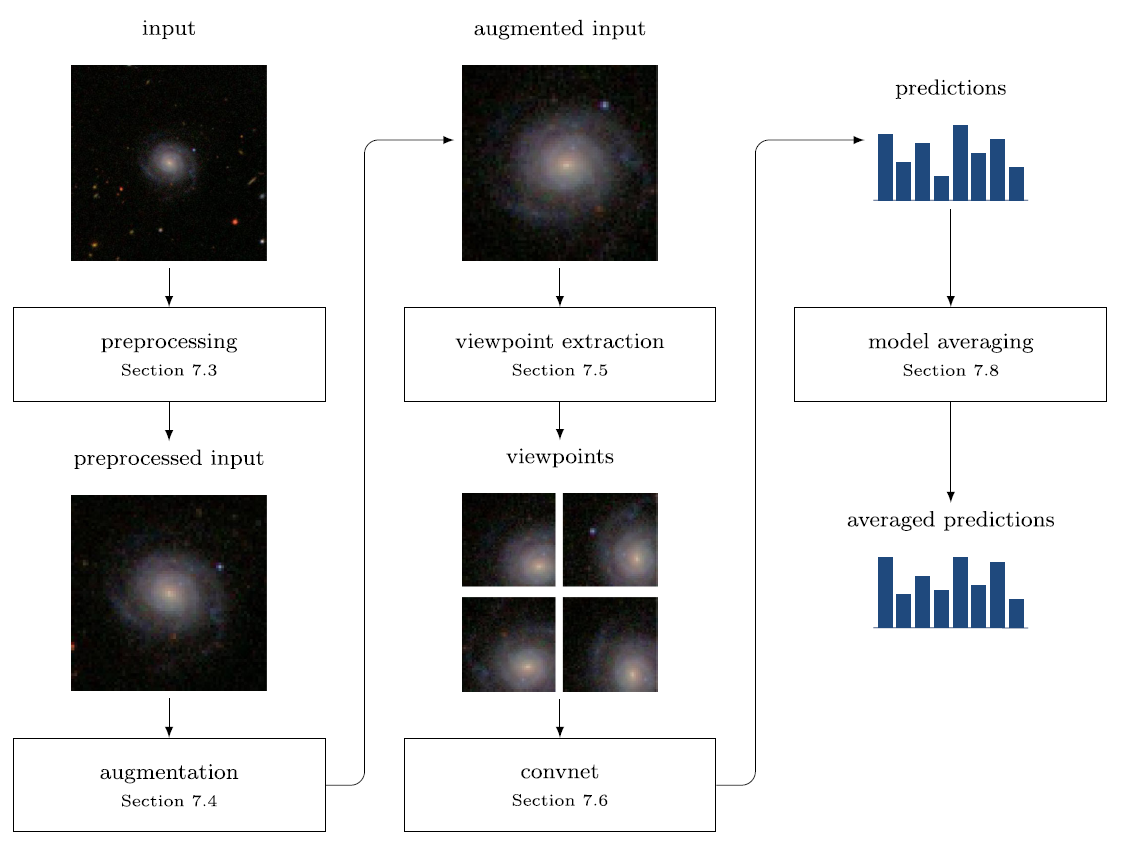
\includegraphics[width=130mm]{../img/GZ2_network.png}
  \caption{Processing pipeline for the top model in the Galaxy Zoo Kaggle competition. From \cite{2015MNRAS.450.1441D}.}
  \label{fig:GZ2_network}
\end{figure}


The winning algorithm was an ensemble method, averaging the results of many different CNNs. In the pre-processing stage, the image was cropped and rescaled several times down to $69 \times 69$ pixel images, which occasionally removed part of the galaxy. In some of their models, they used SExtractor to estimate the position and size of the galaxy, allowing them to center and rescale the galaxies to a standardized size. In addition, gray-scaling was examined, although this lead to worse results.

Due to the limited sample size, the number of images was increased by performing random pertubations, such as rotating, translating, scaling, and flipping, as well adjusting the color brightness on demand so that the model was never trained on the exact image twice. In addition, the number of images was increased by rotating, flipping and cropping each image into 16 different, but overlapping, $45 \times 45$ pixel images respresenting different viewpoints. Each of the 16 images were then passed together through the CNN, which performed several convolutions and pooling before concatenating the results and passing through a few fully connected layers to output the final categorical probabilities. The probabilities were then averaged over 17 models.

Overall, the model did quite well, achieving $\sim 99\%$ accuracy. It stuggled most with the larger angular sized galaxies (more nearby), as well as those that were not radially symmetric.



% =========================================================
% Proposed Work [old]
% =========================================================
\iffalse

\section{The Proposed Work}
As dicussed earlier, the existing systems from the Galaxy Zoo Kaggle challenge do an excellent job of replicating the voting patterns of citizen science volunteers on the Galaxy Zoo 2 dataset. However, it would be useful to develop an automated system based on the large annotated Galaxy Zoo datasets to classify new imagery from other sources using the popular Hubble Tuning Fork scheme. While this can be done to some extent using the kaggle models, it requires cross-correlating expertly annoted images to find the optimal probability cutoffs to transform the probability distributions to Hubble T-types, adding an additional layer of complexity that the machine wasn't required to learn. We will develop a mapping between the two classification schemes and develop such a machine learning system to directly classify images. 

Our model will differ slightly from the format of the Kaggle challenge. The Kaggle Galaxy Zoo challenge formulated the problem as a regression on the class probabilities, defined as the ratio of citizen science volunteers that gave a given galaxy a certain classification. To match the structure of our gold standard Tuning Fork scheme data, we will instead treat this as a classification problem and select only those galaxies whose vote fractions are within our chosen threshold for each Hubble type. This will favor the more nearby galaxies, whose properties the top performing model in the Kaggle competition had a harder time predicting accurately, hopefully leading to an improvement in that regard. In addition, it would serve as a more interactive tool that could serve as a complement to the galaxy classification lab in \emph{Stars, Galaxies, and the Universe}.

Based on prior work, the best approach to galaxy classification appears to be a Deep Convolutional Neural Network. The top image recognition CNNs in recent years have used the inception model \citep{2014arXiv1409.4842S} as a building block in their networks (Figure \ref{fig:inception}). We will follow this trend.

\fi

\begin{figure}[h]
  \centering
	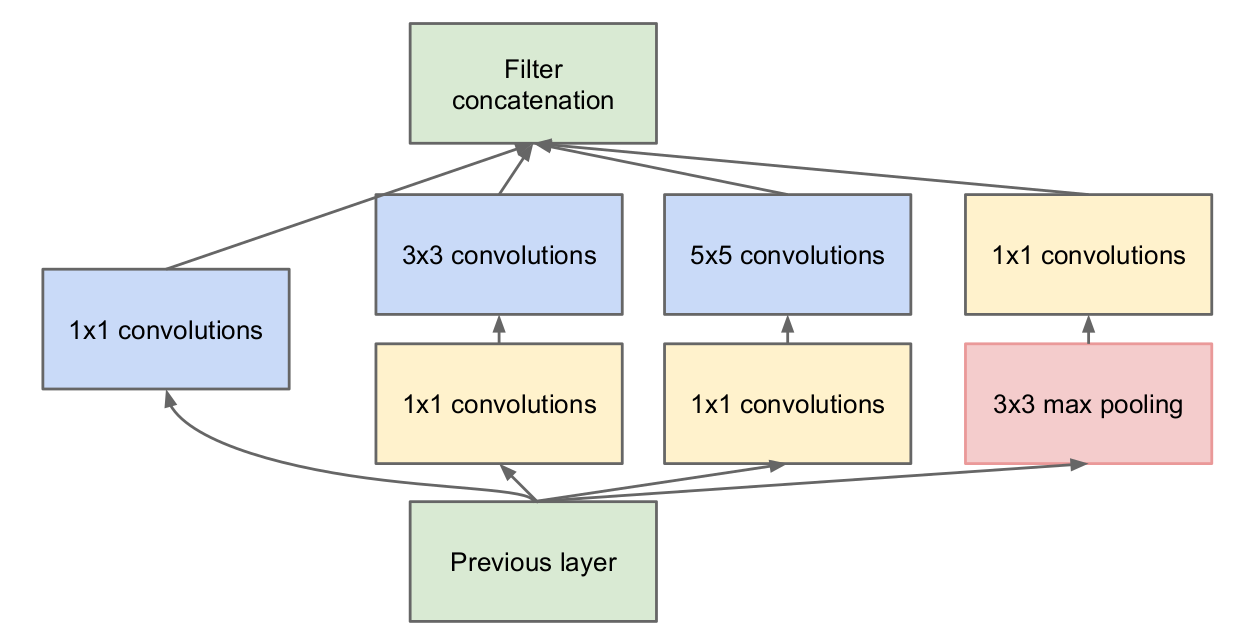
\includegraphics[width=100mm]{../img/inception.png}
  \caption{Inception block. The top image recognition CNNs in recent years use many inception blocks in their networks. From \cite{2014arXiv1409.4842S}.}
  \label{fig:inception}
\end{figure}

\section{Approach}
The existing systems from the Galaxy Zoo 2 Kaggle challenge do an excellent job of replicating the voting patterns of citizen science volunteers on the Galaxy Zoo 2 dataset. Extending this one step further, we developed an automated system trained on the large annotated Galaxy Zoo datasets to classify galaxies directly onto the popular Hubble Tuning Fork scheme. While this can be done to some extent using the kaggle models, it requires cross-correlating expertly annoted images to find the optimal probability cutoffs to transform the probability distributions to Hubble types, adding an additional layer of complexity that the machine wasn’t required to learn.

Our model differs slightly from the format of the Kaggle challenge. The Kaggle Galaxy Zoo challenge formulated the problem as a regression on the class probabilities, defined as the ratio of citizen science volunteers that gave a given galaxy a certain classification. To match the structure of our gold standard Tuning Fork scheme data, we instead treated this as a classification problem and selected only those galaxies whose vote fractions are within our chosen threshold for each Hubble type. This favors the more nearby galaxies, whose properties the top performing model in the Kaggle competition had a harder time predicting accurately. The system might also serve as a more interactive tool that could serve as a complement to the galaxy classification lab in Stars, Galaxies, and the Universe.

Based on prior work, the best approach to galaxy classification appears to be a Deep Convolutional Neural Network. The top image recognition CNNs in recent years have used the inception model \citep{2014arXiv1409.4842S} as a building block in their networks (Figure \ref{fig:inception}). We will follow this trend.

As an initial test, we began with a simple classification system of Ellipticals, Spirals, and Edge-on Spirals using the Galaxy Zoo 1 dataset. Since this dataset contains results for almost 1 million galaxies, we only looked at those that contained only measured redshifts $(\sim 67\%)$, and from those pruned the dataset. Requiring 100\% agreement on Elliptical and Spiral classifications, and $>95\%$ on Edge-on Spirals, we had approximately 4000 galaxies in each category. From these 11845 galaxies, 2200 from each category were sent to a training dataset, 800 to the validation, and the remaining to the testing dataset.

For the Hubble Tuning Fork dataset, we utilized the decision tree results from Galaxy Zoo 2, as well as the expert classifications from \cite{2010ApJS..186..427N}. Since the expert classifications were done according to the de Vaucouleurs system, it is fairly straightfoward to reduce to the Hubble tuning fork system, with the spiral subclasses "ab" and "bc" being classified as "a" and "b" respectively. 

For the GZ2 dataset, the elliptical galaxies were selected from the subset where at least 92.5\% of respondents said the galaxy was smooth. From this subset, the subclass was chosen by the fraction of votes who responded "round", "in between", and "cigar shaped", multiplied by the weights 0.4, 3.5, and 6.75 respectively in an effort to match the subclass distribution from \cite{2010ApJS..186..427N}. The scores were then rounded to the nearest integer.

For the S0 (Lenticular) galaxies, we considered only those cases where >80\% of the respondents said the object was disk-like and from this subset chose only those galaxies where >90\% said the galaxy was viewed edge-on \emph{or} <20\% there were no spiral arms.

For the spirals were required >80\% of respondents to say the galaxy was disk-like, less than 20\% to say the galaxy was edge-on, and >80\% to respond that there were spiral arms present. From these, the regular spirals were chosen from the subset where <10\% of respondents said there was no bar and the barred spirals from the subset where >50\% said there was a bar present. For those in-between, they were dropped from the dataset. The subclasses were chosen by weighting the fraction of votes on the tightness of the spiral arms, assigning weight 0, 1, and 2 to "tight", "medium", and "loose" respectively. The scores were then sorted and split into the three subcategories a, b, and c.

With the classification complete, the galaxy sizes were collected by querying the SDSS database using the mechanize python module. The galaxy sizes were then used to set the image scale, allowing us to fill up most of the image with the galaxy while containing the galaxy within the image. The images were then downloaded using the urllib python module. 60\% of the GZ2 images were sent to the training dataset, and the remaining 40\% split evenly between a validation and testing dataset.


\section{Implementation}
Our galaxy classification model was built on top of Google’s Tensorflow and the open-source deep learning library Keras. Keras has achieved popularity through ease of use and a wide selection of pre-built models. We use the Keras implementation of Google’s Inception V3 architecture, initialized with weights from ImageNet pre-training. Training an Inception model from scratch is computationally intensive. By re-using the ImageNet weights provided by Google, we were able to considerably reduce training time. 

The model was trained for each dataset in two stages. First, the final softmax layer was discarded, and a new softmax layer trained from scratch with all other network weights held constant from the ImageNet initialization. In the second step, the last three layers were retrained for 1000 epochs at a low learning rate (lr=0.001, momentum=0.9) using categorical cross-entropy loss, with all other weights held constant. The classes were weighted to mitigate the large class imbalances. The imagery is already centered and scaled to display the galaxy at a consistent size and location, but additional preprocessing was done to randomly rotate and flip the training images.

Training and testing was done on the University of Iowa ARGON high performance computing cluster. ARGON offers a wide range of compute configurations, including nodes equipped with nVidia workstation class GPU accelerators. For performance reasons, GPU acceleration proved necessary to train the inception model [more specific/what issues?]. 

Four different models were trained on four different datasets.  One model was trained and tested on the Galaxy Zoo 1 dataset. Galaxy Zoo 1 is inadequate for Hubble classification purposes as the available class labels only distinguish whether a galaxy is a spiral, elliptical, or edge-on spiral.  However, there is prior work \cite{2004MNRAS.349...87D} showing 90\% accuracy on classifying the Galaxy Zoo 1 dataset, which allows us to compare the performance of our system to earlier work in the field.

The three remaining models were trained on the Galaxy Zoo 2 dataset (GZ2), the independent expert-labeled dataset (EXP), and a merged Galaxy Zoo 2 and expert-labeled dataset (GS2-EXP). The model build on GZ2 was tested on GZ2 and EXP, the model built on EXP was tested on EXP and the model built on GZ2-EXP was tested on GZ2-EXP and EXP. This allows us to assess the generalization performance of a classifier trained on the Galaxy Zoo 2 dataset when applied to a new dataset, compared to training on the new dataset alone or training after merging the two datasets.

\section{Results}
The system provides excellent performance on GZ1 and is able to generate meaningful predictions on all datasets. On the Galaxy Zoo 1 dataset, we report 95\% classification accuracy, compared to 90\% in previous literature. On Galaxy Zoo 2, we obtain 58\% accuracy and a macro-averaged F1-measure of 0.496. Without retraining, the generalization performance on a new imagery dataset is disappointing at 23\% with a macro-averaged F1-measure at 0.229, but after retraining on a small expert-labeled training set the performance improves to 46\% accuracy and an F1-measure of 0.459. These results show that galaxy classification models trained on the Galaxy Zoo 2 dataset generalize well to other galaxy datasets if a small manually labeled dataset for retraining can be found. 

\begin{table}
\begin{center}
\begin{tabular}{l|c|c|c}
Train/Test	&	GZ1		&	GZ2		&	EXP		\\ \hline
GZ1			&	0.95	&			&			\\
GZ2			&			&	0.58	&	0.23	\\
EXP			&			&			&	0.46
\end{tabular}
\end{center}
\caption{Accuracies for the model trained and evaluated on various testing datasets.}
\end{table}

\begin{table}
\begin{center}
\begin{tabular}{l|c|c|c}
Train/Test	&	GZ2		&	EXP			\\ \hline
GZ2			&	0.496	&	0.229		\\
EXP			&			&	0.459
\end{tabular}
\end{center}
\caption{Macro-averaged F1 measure of the models evaluated on the Hubble classification scheme datasets.}
\end{table}

\section{Future Goals}


\subsubsection*{Acknowledgments}

We would like to acknowledge the work of the Galaxy Zoo team and the countless citizen volunteers in collecting and annotating the massive Galaxy Zoo dataset that makes this work possible. 


\begin{thebibliography}{9}
\bibitem[de la Calleja \& Fuentes(2004)]{2004MNRAS.349...87D} de la Calleja, J., \& Fuentes, O.\ 2004, MNRAS, 349, 87 
\bibitem[Dieleman et al.(2015)]{2015MNRAS.450.1441D} Dieleman, S., Willett, K.~W., \& Dambre, J.\ 2015, MNRAS, 450, 1441
\bibitem[Gaia Collaboration et al.(2016)]{2016A&A...595A...1G} Gaia Collaboration, Prusti, T., de Bruijne, J.~H.~J., et al.\ 2016, Astronomy and Astrophysics, 595, A1  
\bibitem[Gauthier et al.(2016)]{stanford} Gauthier, A., Jain, A., Noordeh, E.\ 2016
\bibitem[Ivezic et al.(2009)]{2009AAS...21346003I} Ivezic, Z., Tyson, J.~A., Axelrod, T., et al.\ 2009, Bulletin of the American Astronomical Society, 41, 460.03 
\bibitem[Kuminski \& Shamir(2016)]{2016ApJS..223...20K} Kuminski, E., \& Shamir, L.\ 2016, ApJS, 223, 20 
\bibitem[Lintott et al.(2008)]{2008MNRAS.389.1179L} Lintott, C.~J., Schawinski, K., Slosar, A., et al.\ 2008, MNRAS, 389, 1179
\bibitem[Nair \& Abraham(2010)]{2010ApJS..186..427N} Nair, P.~B., \& Abraham, R.~G.\ 2010, The Astrophysical Journal Supplement Series, 186, 427 
\bibitem[Skidmore et al.(2015)]{2015RAA....15.1945S} Skidmore, W., TMT International Science Development Teams, \& Science Advisory Committee, T.\ 2015, Research in Astronomy and Astrophysics, 15, 1945 
\bibitem[Szegedy et al.(2014)]{2014arXiv1409.4842S} Szegedy, C., Liu, W., Jia, Y., et al.\ 2014, arXiv:1409.4842 
\bibitem[Willett et al.(2013)]{2013MNRAS.435.2835W} Willett, K.~W., Lintott, C.~J., Bamford, S.~P., et al.\ 2013, MNRAS, 435, 2835  
\end{thebibliography}


\end{document}
